\documentclass{classrep}
\usepackage[utf8]{inputenc}
\usepackage{color}
\usepackage[polish]{babel}
\usepackage[T1]{fontenc}
\usepackage{enumerate}
\usepackage{graphicx}
\usepackage{float}
\restylefloat{table}
\usepackage{multirow}
\usepackage[normalem]{ulem}
\useunder{\uline}{\ul}{}
\selectlanguage{polish}

\studycycle{Informatyka, studia dzienne, I st.}
\coursesemester{VI}

\coursename{Komputerowe systemy rozpoznawania}
\courseyear{2018/2019}

\courseteacher{dr hab. inż. Adam Niewiadomski}
\coursegroup{poniedziałek, 12:15}

\author{
  \studentinfo{Stanisław Zakrzewski}{210360} \and
  \studentinfo{ Maciej Socha}{210321}
}

\title{Zadanie 1: Ekstrakcja cech, miary podobieństwa, klasyfikacja}

\begin{document}
\maketitle

\section{Cel}
Celem zadania było poznanie oraz zaimplementowanie różnych metod ekstrakcji cech z tekstów, określania podobieństwa oraz klasyfikacji tekstów.

\section{Wprowadzenie}
{\color{blue}
We wprowadzeniu należy zaprezentować całą teorię potrzebną do realizacji
zadania (przy czym należy tu ograniczyć się wyłącznie do tego, co było
wykorzystane) tak aby osoba, która nigdy wcześniej nie zetknęła się z tą
tematyką, potrafiła zrozumieć dalszy opis. Część ta powinna wprowadzać
wszystkie wykorzystywane wzory, oznaczenia itp., do których należy się
odwoływać w dalszej części niniejszgo sprawozdania. Zamieszczony tu własny
opis teorii (a nie skopiowany!) należy poprzeć odwołaniami bibliograficznymi
do literatury zamieszczonej na końcu. }

\section{Opis implementacji}
Algorytmy zostały zaimplementowane w języku Java w wersji 11. Dodatkowo na potrzemy procesu lemmatyzacji wykorzystano, udostępnioną przez Stanford Natural Language Processing Group, biliotekę CoreNLP w wersji 3.9.2. Biblioteka ta jest udostępniona z licencją GNU General Public License v3 co pozwala nam korzystać z niej w naszym programie. Biblioteka ta jest bardzo obszerna, w naszym programie wykorzystujemy jedynie funkcjonalność lemmatyzacji. Jest ona zaimplementowana w klasie StanfordLemmatizer. Implementacja tej klasy została bezpośrednio zaczerpnięta z dokumentacji[5]. Poniżej przedstawiono uproszczony diagram klas. Zaznaczone zostały na nim kluczowe dla działania naszego programu klasy.\\
{\color{red}
Tutaj diagramy uml wraz z podpisami\\}

\begin{figure}[H]
	\makebox[\linewidth]{
		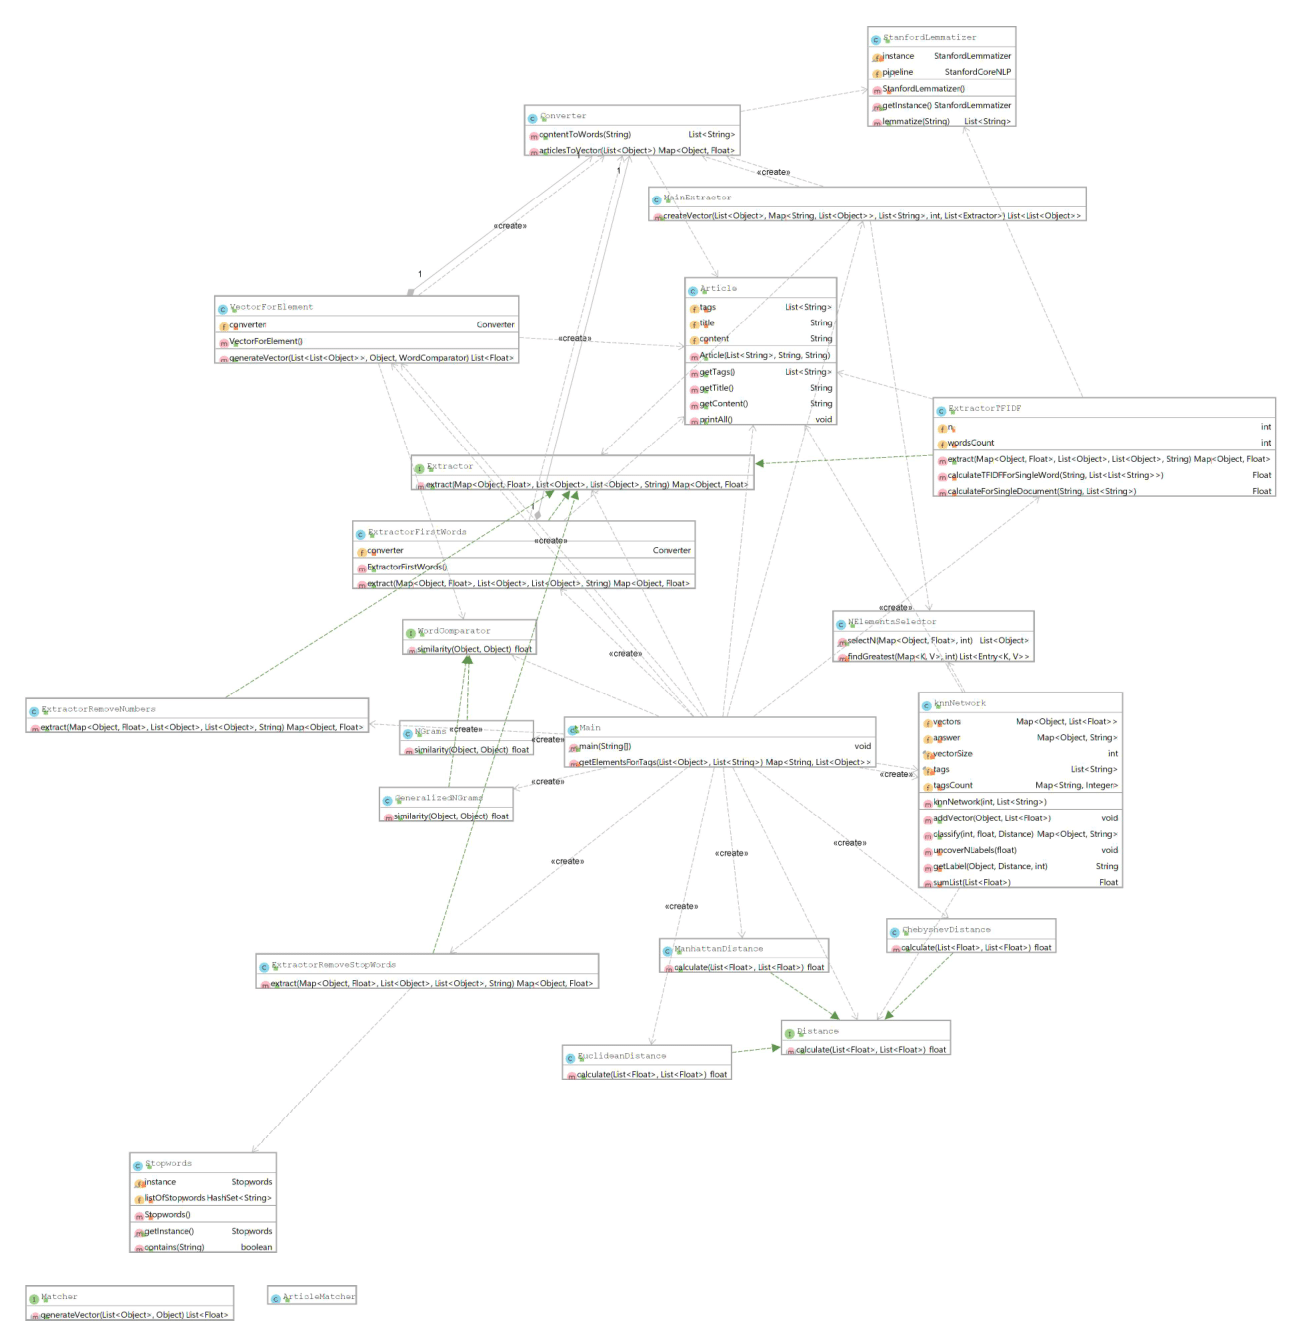
\includegraphics[scale=0.2]{uml.png}
	}
	\caption{UML Diagram}
\end{figure}

Klasa Article odpowiada za przechowywanie informacji niezbędnych do działania programu. Wykorzystujemy ją zarówno do przetwarzania artukułów zawartych w zbiorze danych reuters jak i zestawu artykułów przygotowanego przez nas samych.\\
Interfejs Extractor służy i znajdująca się w nim metoda extract jest wykorzystywana przy procesie ekstakcji cech. Implementują ją liczne klasy zawierające sie w dwóch sposobach ekstarakcji cech zawartych w programie.\\
Klasa knnNetwork zawiera w sobie implementację algorytmu k najbliższych sąsiadów do ustalania przynależności wektorów odpowiadającycm przekazanym do programu elementom. Klasa pozwala na dodawanie wektorów wraz z odpowiadającymi im elementami, a następnie klasyfikowanie ich przy przekazaniu odpowiedniego parametru k oznaczającego liczbę sąsiadów, uncoveredLabelFraction zapomocą którego przekazujemy jaka część tekstów będzie miała odkryte etykiety oraz distance, metrykę obliczania dystansu pomiędzy wektorami.\\
Pakiet calculatedistance zawiera w sobie interfejs Distance oraz implementujące go klasy ChebyshevDistance(metryka Czebyszewa), EuclideanDistance(metryka Euklidesa) oraz ManhattanDistance(metryka uliczna). Są to wymagane przez treść zadania metryki pomiaru odległości pomiędzy wektorami.\\
Za przekazywanie danych do programu odpowiada plik config.txt zawierający w sobie wszystkie potrzebne do działania programu parametry. Są to odpowiednio:
\begin{enumerate}
	\item tagClass - tag dla którego etykiety będzie nadawał program
	\item folderPath - ścieżka do folderu z plikami z danymi
	\item articlesToReadCount - liczba plików z artykułami, które program ma wczytać
	\item tags - etykiety, według których program ma klasyfikować
	\item numberOfElementsPerTag - liczba elementów jakie ma zawierać w sobie cecha dla każdej z etykiet
	\item trainToTestRatio - stosunek zbioru treningowego do testowego
	\item distanceKNN - metryka pomiaru dystansu w przestrzeni dla algorytmu knn
	\item wordSimilarity - metryka podobieństwa słów
	\item extractors - zestaw ekstraktorów
\end{enumerate}

{\color{blue}
Należy tu zamieścić krótki i zwięzły opis zaprojektowanych klas oraz powiązań
między nimi. Powinien się tu również znaleźć diagram UML  (diagram klas)
prezentujący najistotniejsze elementy stworzonej aplikacji. Należy także
podać, w jakim języku programowania została stworzona aplikacja. }

\section{Materiały i metody}
{\color{blue}
W tym miejscu należy opisać, jak przeprowadzone zostały wszystkie badania,
których wyniki i dyskusja zamieszczane są w dalszych sekcjach. Opis ten
powinien być na tyle dokładny, aby osoba czytająca go potrafiła wszystkie
przeprowadzone badania samodzielnie powtórzyć w celu zweryfikowania ich
poprawności (a zatem m.in. należy zamieścić tu opis architektury sieci,
wartości współczynników użytych w kolejnych eksperymentach, sposób
inicjalizacji wag, metodę uczenia itp. oraz informacje o danych, na których
prowadzone były badania). Przy opisie należy odwoływać się i stosować do
opisanych w sekcji drugiej wzorów i oznaczeń, a także w jasny sposób opisać
cel konkretnego testu. Najlepiej byłoby wyraźnie wyszczególnić (ponumerować)
poszczególne eksperymenty tak, aby łatwo było się do nich odwoływać dalej.}

\section{Wyniki}
{\color{blue}
W tej sekcji należy zaprezentować, dla każdego przeprowadzonego eksperymentu,
kompletny zestaw wyników w postaci tabel, wykresów itp. Powinny być one tak
ponazywane, aby było wiadomo, do czego się odnoszą. Wszystkie tabele i wykresy
należy oczywiście opisać (opisać co jest na osiach, w kolumnach itd.) stosując
się do przyjętych wcześniej oznaczeń. Nie należy tu komentować i interpretować
wyników, gdyż miejsce na to jest w kolejnej sekcji. Tu również dobrze jest
wprowadzić oznaczenia (tabel, wykresów) aby móc się do nich odwoływać
poniżej.}

\section{Dyskusja}
{\color{blue}
Sekcja ta powinna zawierać dokładną interpretację uzyskanych wyników
eksperymentów wraz ze szczegółowymi wnioskami z nich płynącymi. Najcenniejsze
są, rzecz jasna, wnioski o charakterze uniwersalnym, które mogą być istotne
przy innych, podobnych zadaniach. Należy również omówić i wyjaśnić wszystkie
napotakane problemy (jeśli takie były). Każdy wniosek powinien mieć poparcie
we wcześniej przeprowadzonych eksperymentach (odwołania do konkretnych
wyników). Jest to jedna z najważniejszych sekcji tego sprawozdania, gdyż
prezentuje poziom zrozumienia badanego problemu.}

\section{Wnioski}
{\color{blue}W tej, przedostatniej, sekcji należy zamieścić podsumowanie
najważniejszych wniosków z sekcji poprzedniej. Najlepiej jest je po prostu
wypunktować. Znów, tak jak poprzednio, najistotniejsze są wnioski o
charakterze uniwersalnym.}


\begin{thebibliography}{0}
  \bibitem{article1} David D. Lewis.
  	\textsl{Feature Selection and Feature Extract ion for Text Categorization}, University of Chicago,\\
  	Dostępny w Internecie: \url {https://aclweb.org/anthology/H92-1041?fbclid=IwAR248ftiyFqXrFpi51IDLorT7Ngso369BPTOaOeSYE3QGG1gYD9TNfy58qc}

  \bibitem{article2} David Dolan Lewis.
  	\textsl{Representation and learning in information retrieval}, University of Massachusetts,\\
  	Dostępny w Internecie: \url {http://ciir.cs.umass.edu/pubfiles/UM-CS-1991-093.pdf}

  \bibitem{article3} David D. Lewis.
  	\textsl{Data Extraction as Text Categorization : An
Experiment With the MUC-3 Corpus}, University of Chicago,\\
	Dostępny w Internecie: \url {https://www.aclweb.org/anthology/M91-1035}

  \bibitem{article4} Marina Sokolova, Guy Lapalme.
  	\textsl{A systematic analysis of performance measures for classification tasks}, Information Processing and Management no 45,\\
  	Dostępny w internecie: \url {http://rali.iro.umontreal.ca/rali/sites/default/files/publis/SokolovaLapalme-JIPM09.pdf?fbclid=IwAR2M7_a4QxL_F4yCOB_Akp4ghkoUKrBnHT9xzCfuTcoVrLBe3lN3kIlPt00}

  \bibitem{stanford} \url {https://stanfordnlp.github.io/CoreNLP}

\end{thebibliography}
{\color{blue} 
\end{document}
